
% \begin{frame}{\small For example, consider the following \textbf{TPS} configuration,}
%     \vspace*{-0.2in}
%     \footnotesize
%     \begin{center}
%         \centering
%         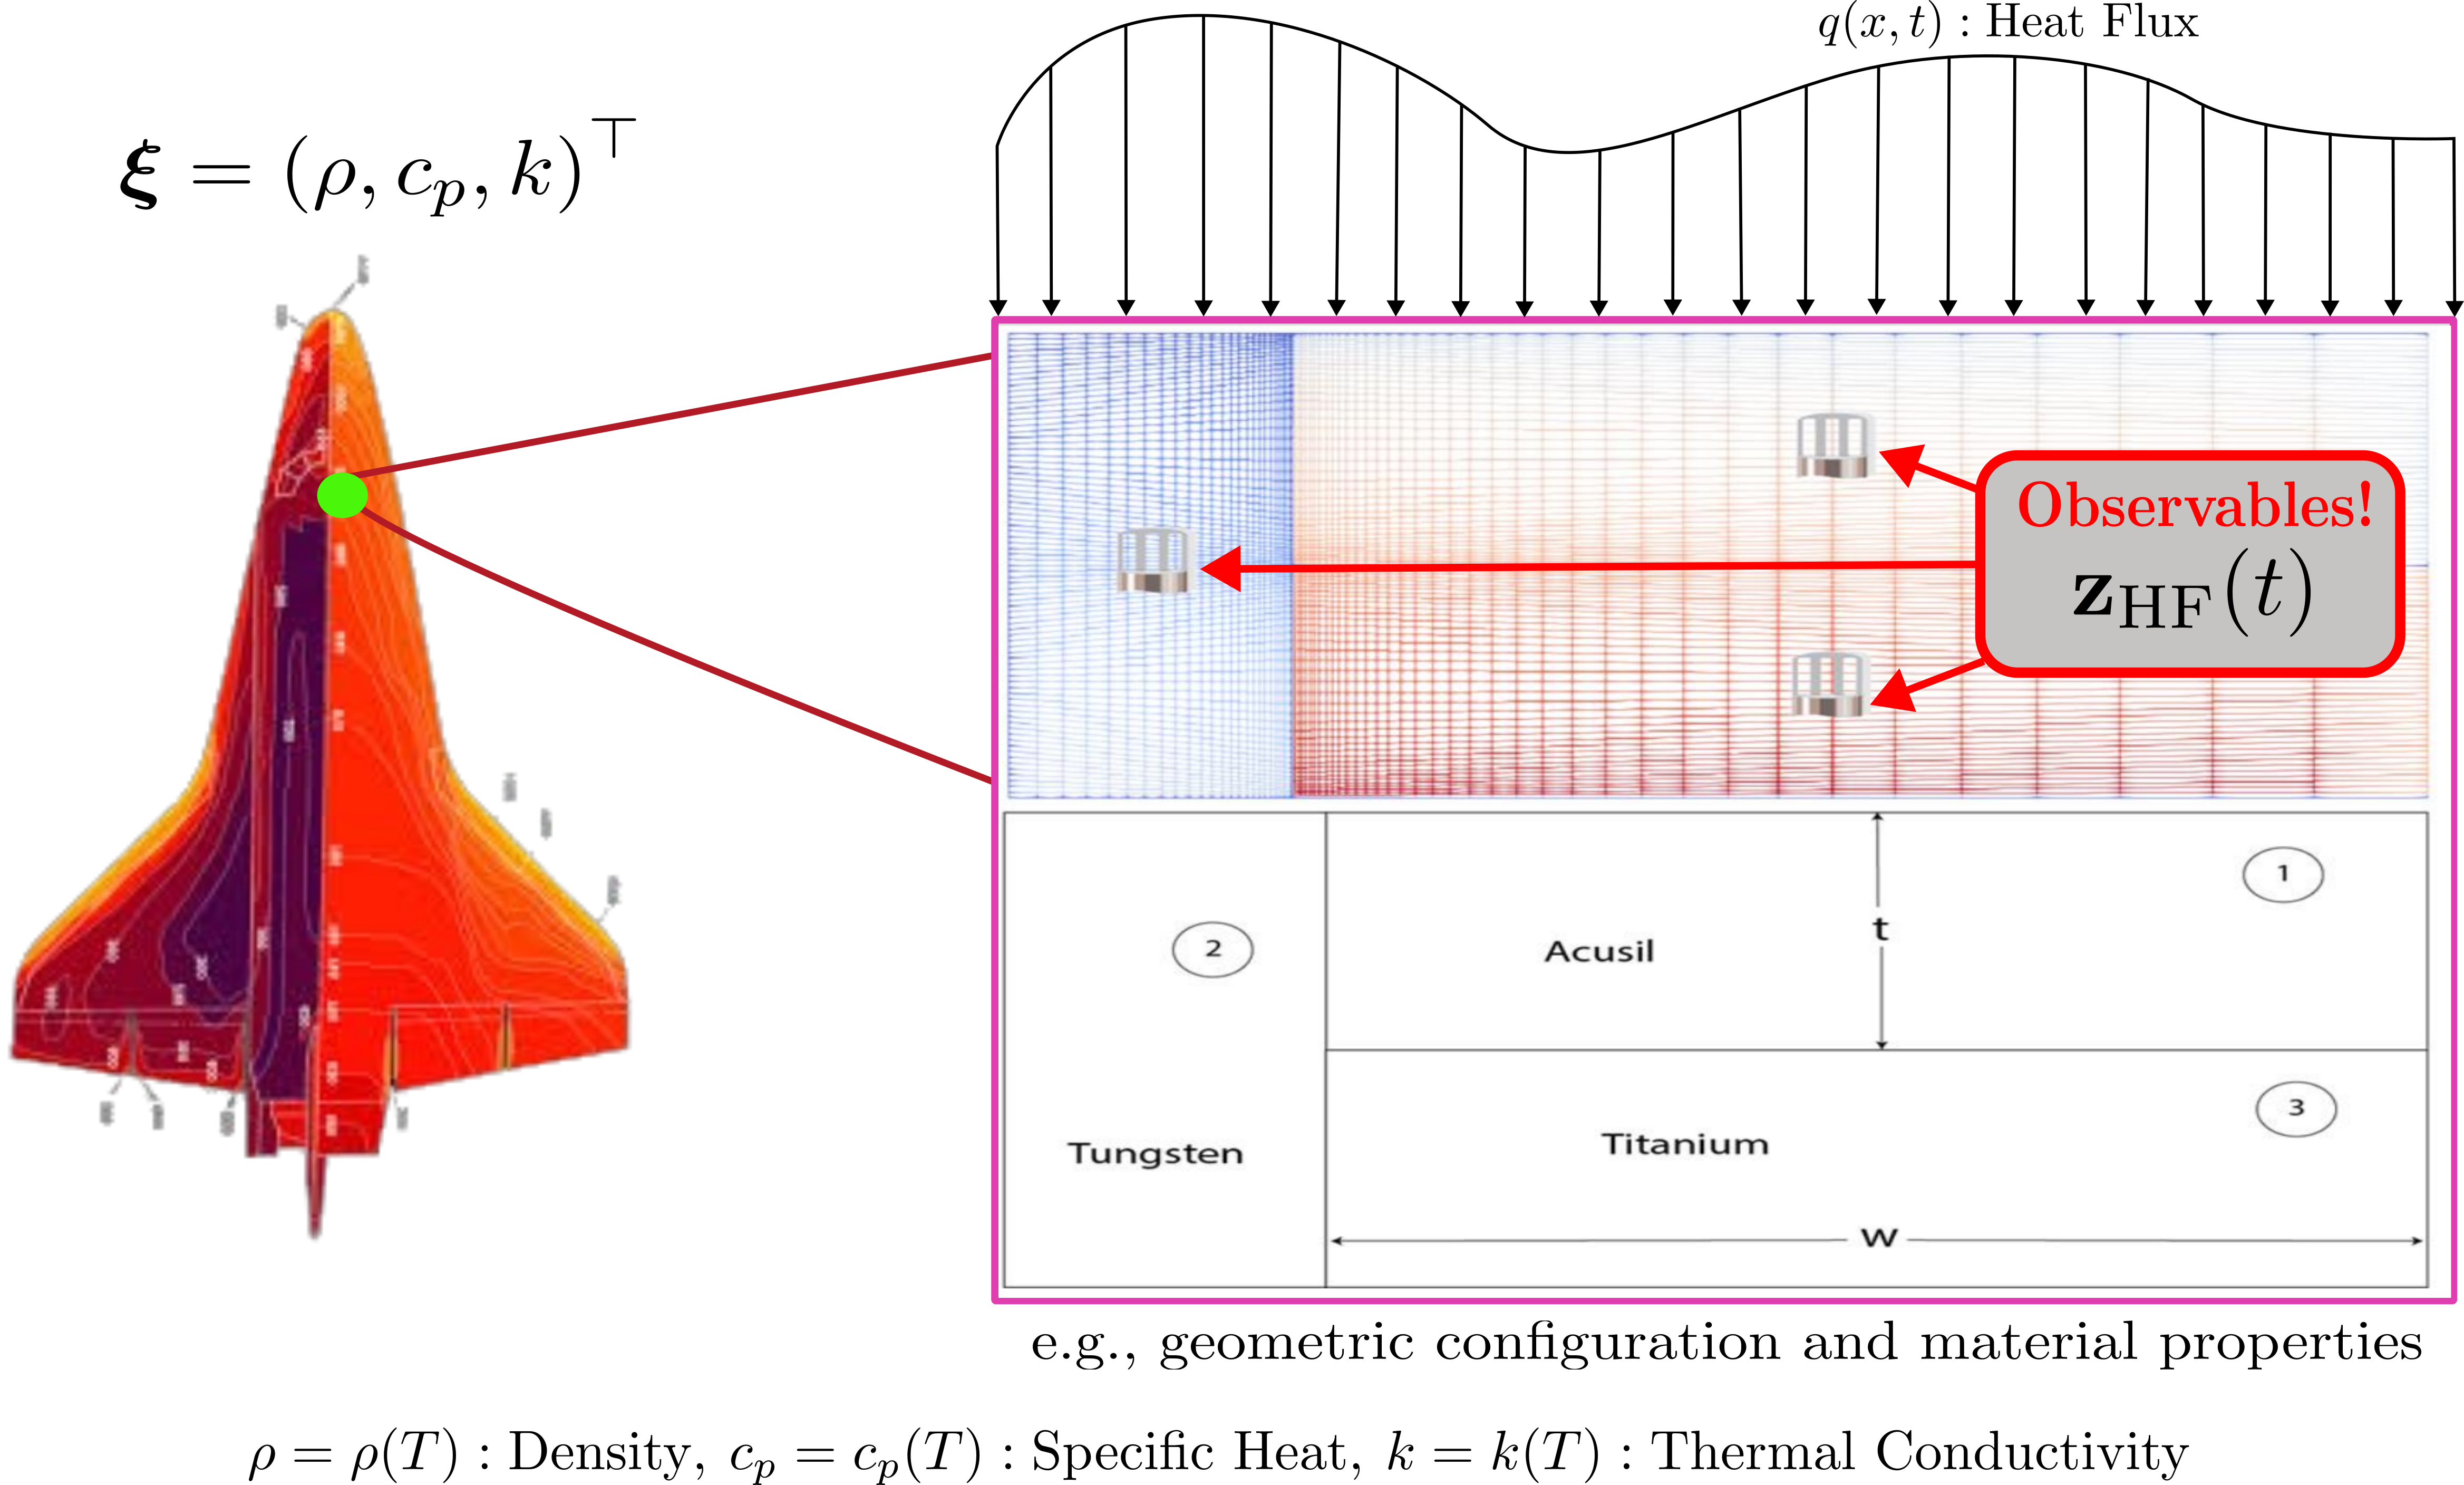
\includegraphics[width=0.7\textwidth]{../figs/pirom/tps.png}
%     \end{center}
%     \begin{center}
%         {\tiny TPS: thermal protection system}
%     \end{center}
% \end{frame}

\begin{frame}{\small For example, consider the following \textbf{TPS} parametrization,}
    \vspace*{-0.2in}
    \footnotesize
    \only<2>{
        \begin{figure}
            \centering
            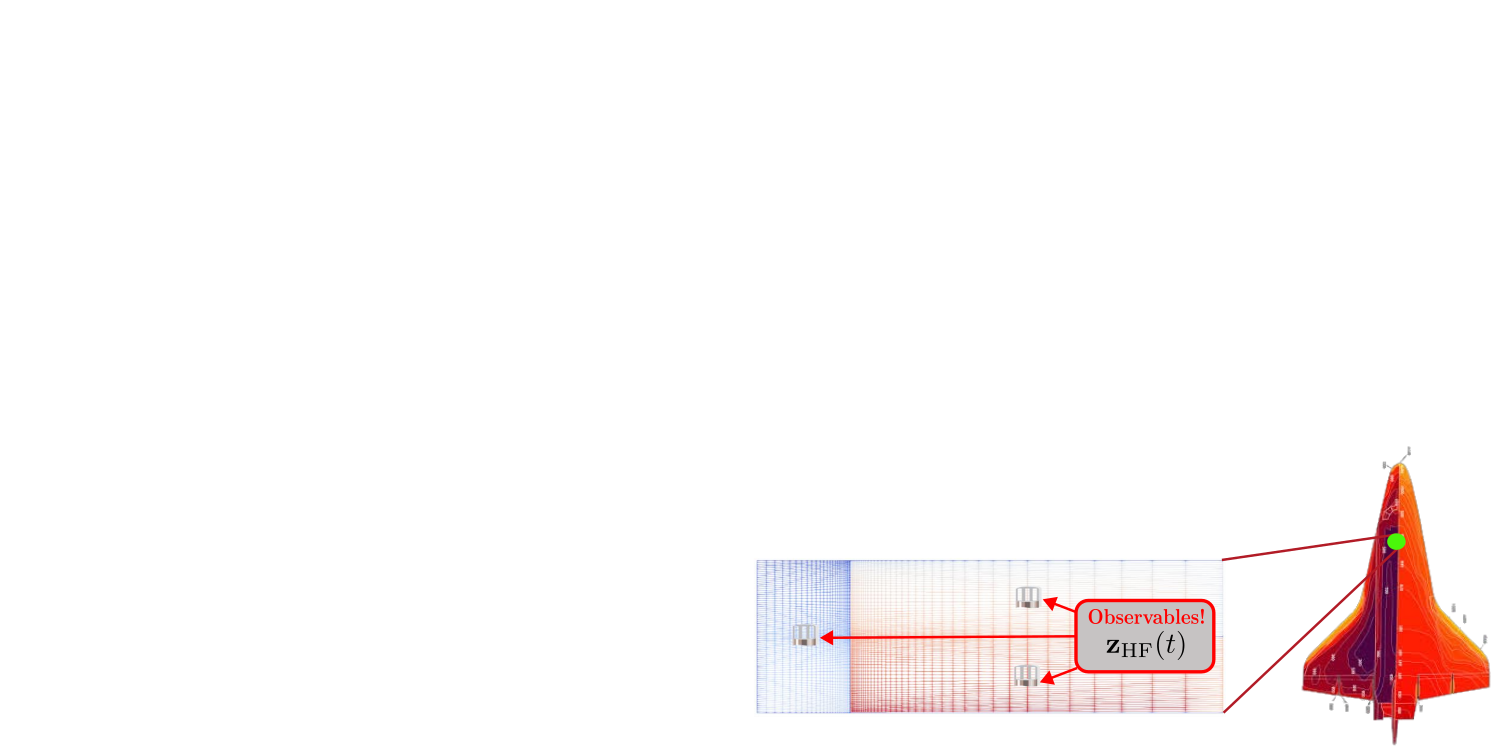
\includegraphics[width=0.9\textwidth]{../figs/pirom/tps_data_1.png}
        \end{figure}}
    \only<3>{
        \begin{figure}
            \centering
            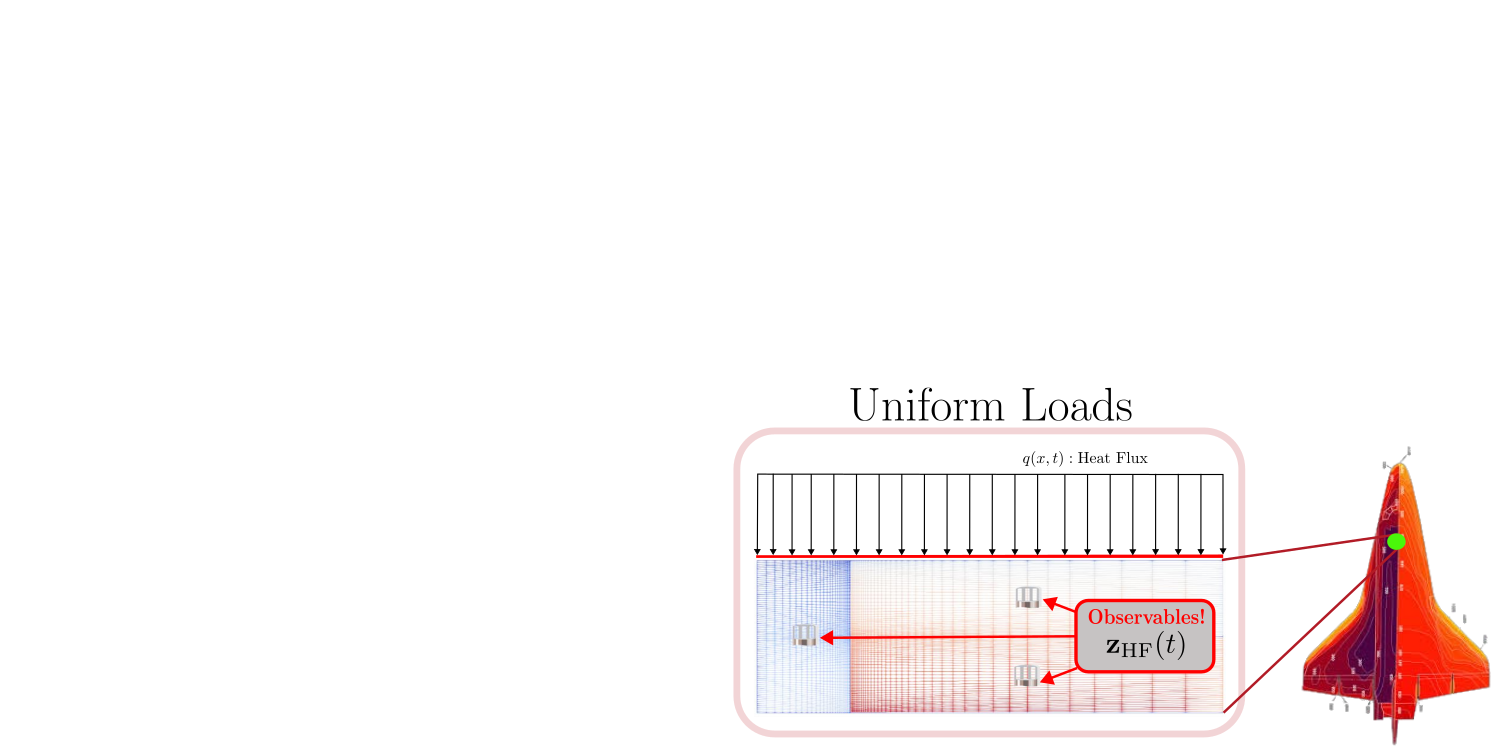
\includegraphics[width=0.9\textwidth]{../figs/pirom/tps_data_2.png}
        \end{figure}}
    \only<4>{
        \begin{figure}
            \centering
            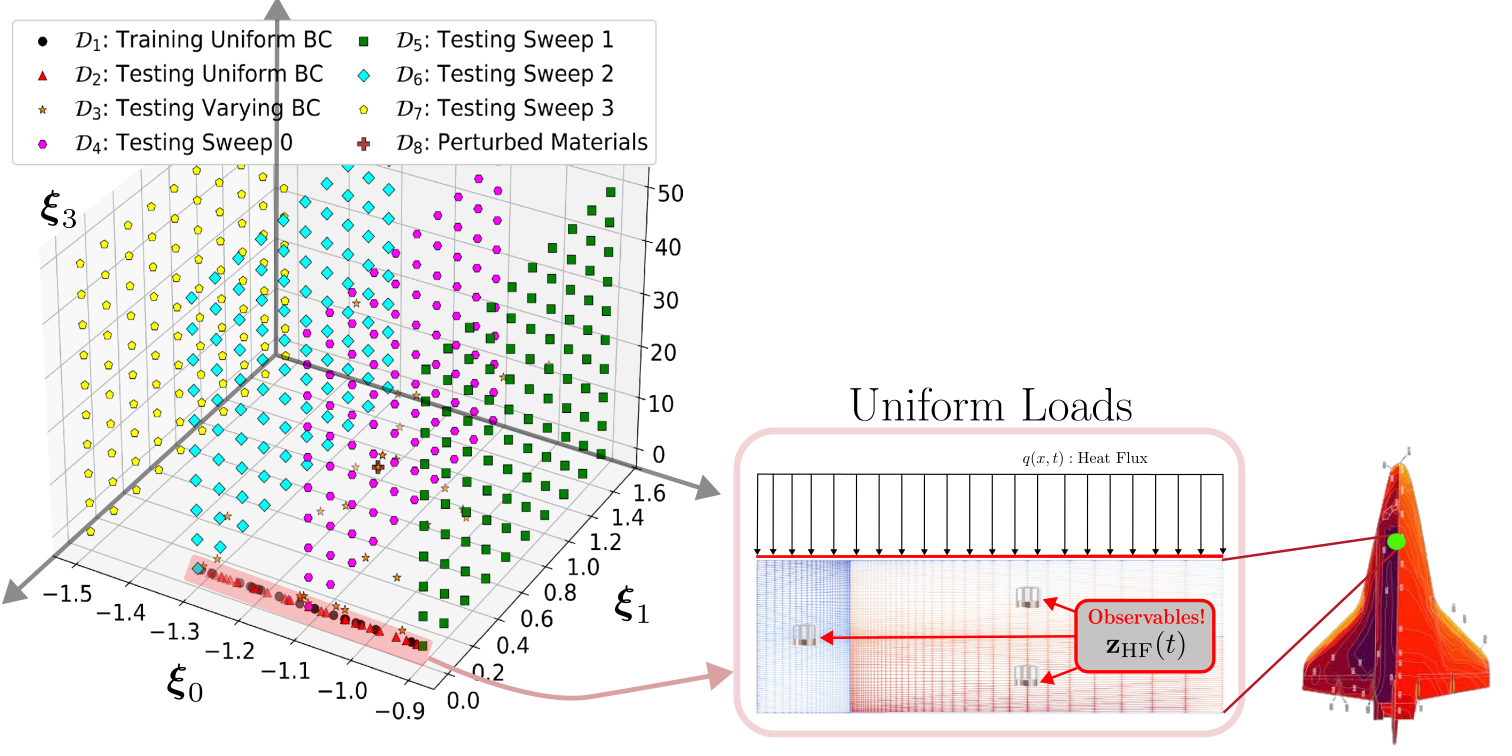
\includegraphics[width=0.9\textwidth]{../figs/pirom/tps_data_3.png}
        \end{figure}}
    \only<5>{
        \begin{figure}
            \centering
            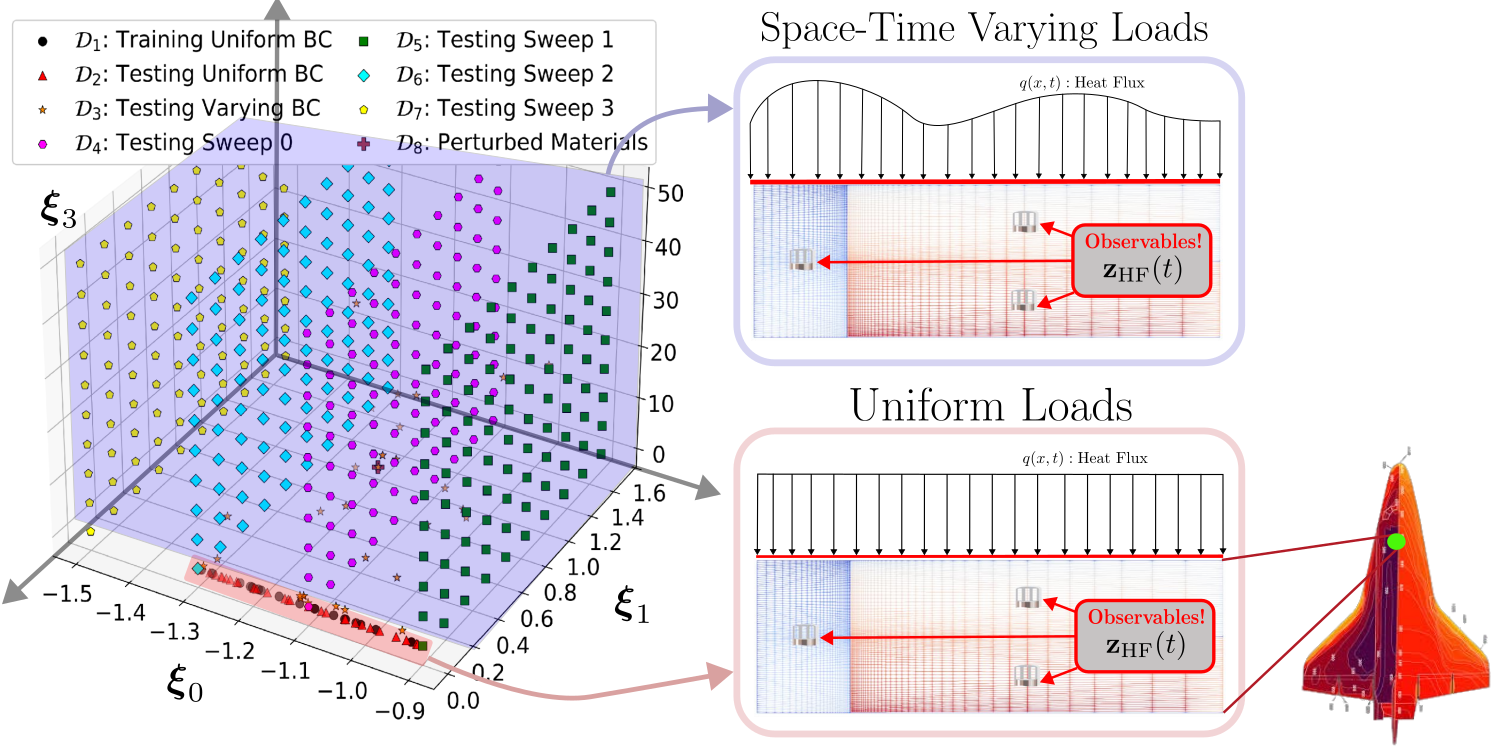
\includegraphics[width=0.9\textwidth]{../figs/pirom/tps_data_4.png}
        \end{figure}}
    \only<6>{
        \begin{figure}
            \centering
            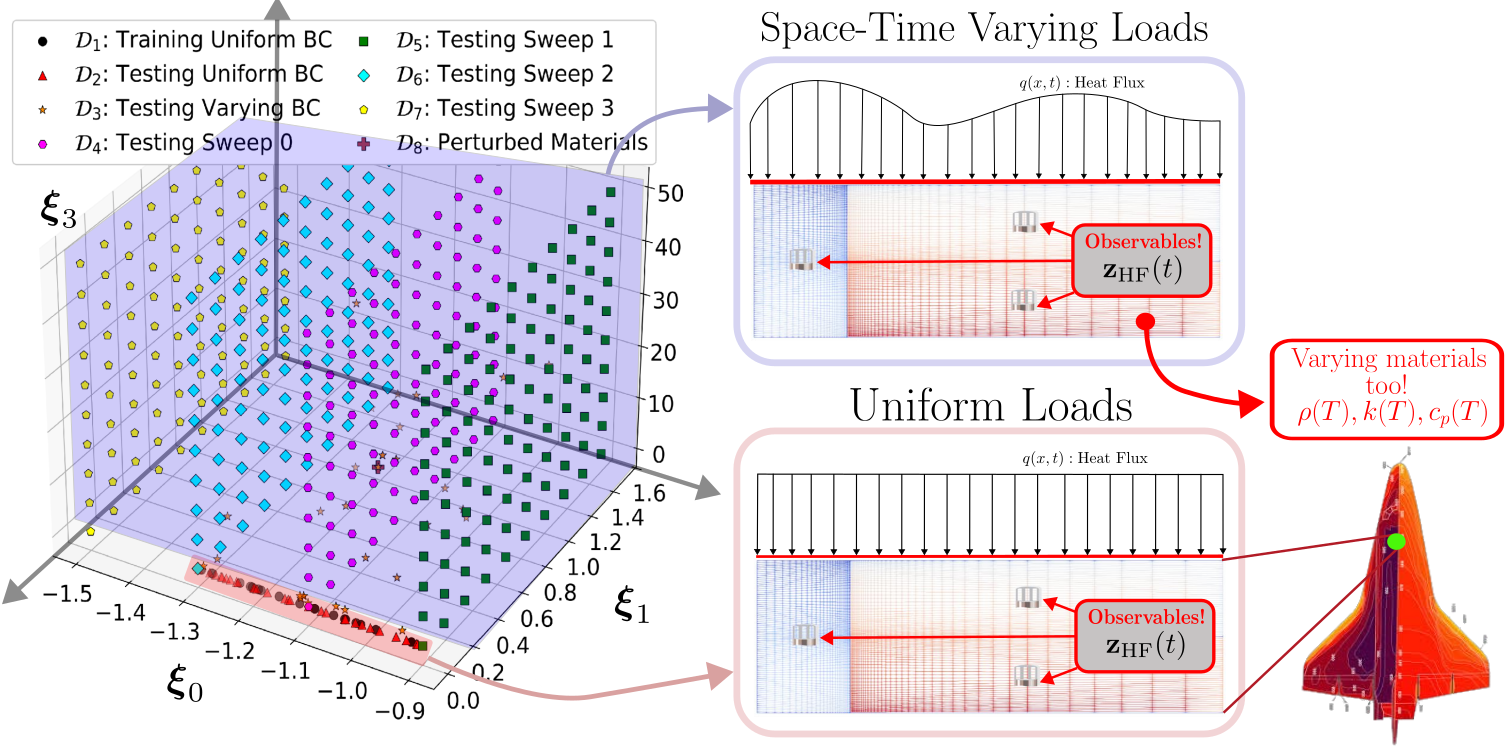
\includegraphics[width=0.9\textwidth]{../figs/pirom/tps_data_5.png}
        \end{figure}}
    \visible<2->{
    \begin{center}
        {\tiny TPS: thermal protection system}
    \end{center}}
\end{frame}

% \begin{frame}{\small \textbf{Quantify} the impossible trinity of modeling (ITM),}
%     \vspace*{-0.2in}
%     \footnotesize
%     \begin{columns}
%         \visible<2->{
%         \begin{column}{0.35\textwidth}
%             \vspace*{0.3in}
%             \begin{figure}
%                 \centering
%                 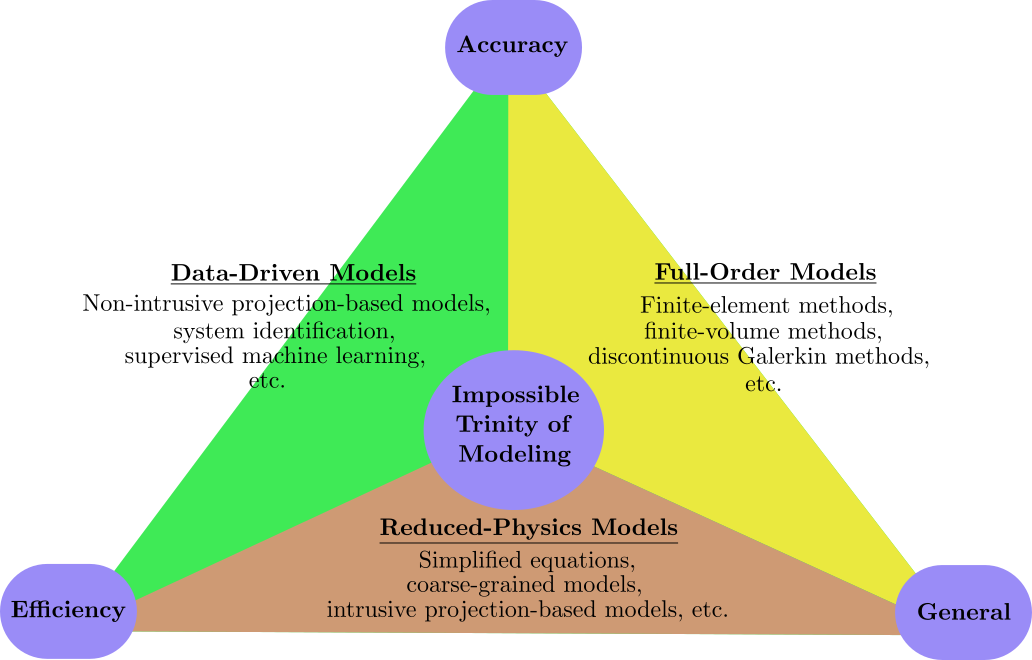
\includegraphics[width=0.9\textwidth]{../figs/introduction/itm.png}
%             \end{figure}}
%         \end{column}
%         \hspace*{-0.2in}
%         \begin{column}{0.7\textwidth}
%             \centering
%             \begin{itemize}
%                 \visible<3->{
%                 \item \textbf{Accuracy}: normalized root mean square error (NRMSE),
%                 \begin{equation*}
%                     e_u^{(l)} = \frac{1}{\Delta z_{u,\text{HF}}^{(l)}}\sqrt{\frac{1}{p}\sum_{k=0}^{p-1}\left(z_{u,\text{HF}}^{(l)}(t_k) - z_{u,\text{ROM}}^{(l)}(t_k)\right)^2}
%                 \end{equation*}}
%                 \visible<4->{
%                 \item \textbf{Efficiency}: \textcolor{blue}{acceleration} ($\mathcal{A}$) and \textcolor{red}{overhead} ($\mathcal{O}$) factor,
%                 \begin{equation*}
%                     \mathcal{A} = \frac{\mathcal{T}^{\text{predict}}_{\text{HF}}(\mathcal{D})}{\mathcal{T}^{\text{predict}}_{\text{ROM}}(\mathcal{D})},\quad \mathcal{O} = \frac{\mathcal{T}^{\text{train}}_{\text{ROM}}(\cD)}{\mathcal{T}^{\text{predict}}_{\text{HF}}(\cD)}
%                 \end{equation*}}
%                 \visible<5->{
%                 \item \textbf{Generalizability}: unseen BCs and materials,
%                 \begin{equation*}
%                     \text{(\textcolor{red}{difficult for ROMs in small data regimes!})}
%                 \end{equation*}}
%             \end{itemize}
%         \end{column}
%     \end{columns}
%     \vspace{-0.28in}
%     \begin{center}
%         \tiny $\mathcal{T}_{\text{HF}}$: FOM wall-clock time, $\mathcal{T}_{\text{ROM}}$: ROM wall-clock time, $\Delta z_{i,\text{HF}}^{(l)}$: range of HF observables
%     \end{center}
% \end{frame}

\begin{frame}{\small Is PIROM any better than the \textbf{SoTA} in small data regimes?}
    \vspace*{-0.3in}
    \footnotesize
    \only<2>{
    \begin{figure}
        \centering
        
\includegraphics[width=1.05\textwidth]{../figs/pirom/performance_1.png}
    \end{figure}}
    \only<3>{
    \begin{figure}
        \centering
        
\includegraphics[width=1.05\textwidth]{../figs/pirom/performance_2.png}
    \end{figure}}
    \only<4>{
    \begin{figure}
        \centering
        
\includegraphics[width=1.05\textwidth]{../figs/pirom/performance_3.png}
    \end{figure}}
    \only<5>{
    \begin{figure}
        \centering
        
\includegraphics[width=1.05\textwidth]{../figs/pirom/performance_4.png}
    \end{figure}}
    \only<6>{
    \begin{figure}
        \centering
        
\includegraphics[width=1.05\textwidth]{../figs/pirom/performance_5.png}
    \end{figure}}
    \visible<2->{
    \begin{center}
        {\tiny NODE: neural ordinary differential equations, OpInf: operator inference, NRMSE: normalized root mean square error, SoTA: state-of-the-art}
    \end{center}}
\end{frame}

% \begin{frame}{\small Is the Impossible Trinity of Modeling \textbf{solved}?}
%     \footnotesize
%     \begin{columns}
%         \visible<1->{
%         \begin{column}{0.3\textwidth}
%             \vspace*{0.3in}
%             \centering
%             \begin{figure}
%                 \centering
%                 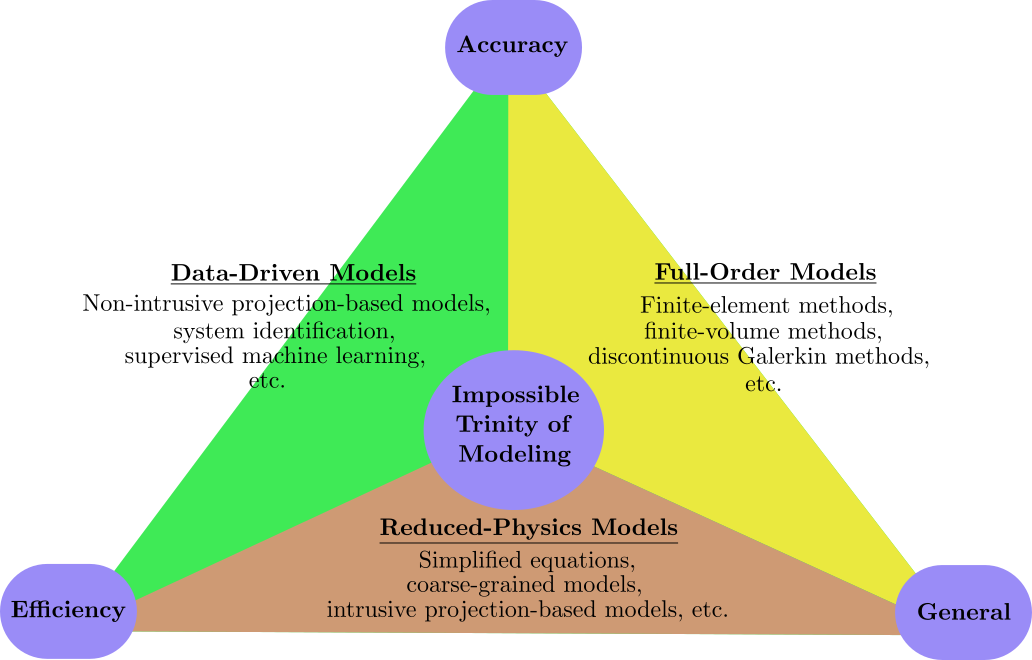
\includegraphics[width=0.9\textwidth]{../figs/introduction/itm.png}
%             \end{figure}
%         \end{column}}
%         \begin{column}{0.8\textwidth}
%             \centering
%             \begin{itemize}
%                 \item<2-> \textbf{Accuracy}: comparable to FOMs (NRMSE $<1\%$),
%                 \item<3-> \textbf{Efficiency}: two-to-three orders of magnitude faster than FOMs,
%                 \item<6-> \colorbox{green!30}{\textbf{Generalizability}}:
%                 \begin{itemize}
%                     \item<7-> \colorbox{green!30}{\textbf{Dimensions}: un-seen loading conditions},
%                     \item<8-> \colorbox{green!30}{\textbf{Physics}: un-seen material properties} 
%                 \end{itemize}
%                 \visible<9->{
%                 \item \textbf{What about training efficiency?}}
%                 \begin{itemize}
%                     \item<10-> \textbf{Overhead} is \colorbox{red!30}{$\approx$ 4 hrs in 3 CPUs} (similar to NODE),
%                     \item<12-> therefore, we need to explore \colorbox{red!30}{other training approaches!}
%                 \end{itemize}
%             \end{itemize}
%         \end{column}
%     \end{columns}
%     \visible<2->{
%     \begin{tikzpicture}[remember picture, overlay]
%         \node[anchor=north west, xshift=1.97cm, yshift=-2.9cm] at (current page.north west) {
\includegraphics[width=0.05\textwidth]{../figs/pirom/checkmark.png}};
%     \end{tikzpicture}}
%     \visible<3->{
%     \begin{tikzpicture}[remember picture, overlay]
%         \node[anchor=north west, xshift=0.34cm, yshift=-4.95cm] at (current page.north west) {
\includegraphics[width=0.05\textwidth]{../figs/pirom/checkmark.png}};
%     \end{tikzpicture}}
%     \visible<6->{
%     \begin{tikzpicture}[remember picture, overlay]
%         \node[anchor=north west, xshift=3.65cm, yshift=-4.95cm] at (current page.north west) {
\includegraphics[width=0.05\textwidth]{../figs/pirom/checkmark.png}};
%     \end{tikzpicture}}
% \end{frame}